\documentclass[spanish]{article}

%% Language and font encodings
\usepackage[spanish]{babel}
\selectlanguage{spanish}
\usepackage[utf8]{inputenc}

%% Sets page size and margins
\usepackage[top=3cm,bottom=2cm,left=3cm,right=3cm,marginparwidth=1.75cm]{geometry}

%% Useful packages
\usepackage{amsmath}
\usepackage{amsfonts}
\usepackage{graphicx}
\usepackage[colorinlistoftodos]{todonotes}
\usepackage[colorlinks=true, allcolors=blue]{hyperref}
\usepackage{apacite}
\usepackage{caption} 
\captionsetup[table]{skip=10pt}

\title{Proyecto Máquinas de Aprendizaje Computacional: \\
	\large{Predicción de Incendios Forestales utilizando técnicas de Máquinas de Aprendizaje}}
  \author{Daniel San Martín \\ 
	\texttt{daniel.sanmartinr@sansano.usm.cl}
}

\date{\today}

\begin{document}
	\renewcommand{\BOthers}[1]{et al.\hbox{}}
	
  \maketitle
    
  \section{Introducción}

    Los incendios forestales son unos de los problemas medioambientales de mayor interés por el daño que generan
    en términos económicos, ambientales y por poner en peligro vidas humanas. Es por esto último que poder modelar
    estos fenómenos se convierte en una tarea de vital importancia. \medskip
    
    Según \cite{preisler2013forest} los modelos de incendios se pueden agrupar en tres tipos: los modelos de riesgo, de 
    propagación y de efecto. Los primeros están asociados a cuantificar la probabilidad y potenciales efectos ante 
    posibles episodios de incendio. Según las variables utilizadas se pueden encontrar distintos trabajos como por ejemplo
    la estimación de la probabilidad de ocurrencia de un incendio en función de la ubicación y el día del año 
    \cite{brillinger2003risk,hernandez2010integrating}, peligro de incendio e índices climáticos \cite{van1987development,
    burgan19881988} entre otros \cite{braun2010forest,ager2007modeling,calkin2011comparative}. El segundo grupo intenta 
    modelar la propagación del fuego y existen desde enfoques físicos \cite{rothermel1972mathematical} hasta modelos de 
    regresión para estimar la tasa de propagación \cite{sullivan2009wildland}. Generalmente este tipo de modelos asume que 
    el combustible (lugar donde ocurre el incendio) puede ser teselado por una malla regular en donde cada celda tiene 
    asociada una probabilidad de quemarse y que depende de las condiciones de las celdas vecinas. Existen distintas 
    herramientas asociadas a este tipo de modelos y pueden ser revisados en \cite{andrews1986behave,finney2006overview,
    finney1998farsite,finney2011simulation,finney2011method}. Por último, los modelos de efecto son importantes
    para estudiar la administración y gestión de los combustibles, por ejemplo el control de mortalidad de árboles 
    o análisis de ecosistemas, entre otros \cite{Larkin-2009,reinhardt2003using,robichaud2007predicting}. \medskip
    
    El desarrollo de este trabajo se basará en el artículo \cite{cortez} que realiza una comparación entre distintos 
    modelos de \emph{Aprendizaje de Máquinas} para predecir el comportamiento de un incendio dado datos meteorológicos. 
    Además se espera incluir una propuesta de modelo utilizando un \emph{Ensamblado de Máquinas} para intentar mejorar 
    la calidad de los resultados. 
            

	\subsection{Datos}
    
  	Para el desarrollo de este proyecto se utilizará el \emph{dataset} ``Forest Fires Data Set'' del 
    \emph{UCI Machine Learning Repository} \cite{cortez} y las características generales del \emph{dataset} 
    están descritas en el Cuadro~\ref{tab:features}.
    
    \clearpage
    
    \begin{table}[!ht]
    	\centering            
      \caption{Características de los datos}
    	\begin{tabular}{ll} 
      	\hline
      	Características de los datos & Multivariados \\              			    				
        Características de los atributos & Reales y Etiquetas \\
        Tareas asociadas & Regresión \\
        Número de instancias & 517 \\
        Número de atributos & 13 \\
        Área & Física \\
        Fecha donación & 2008-02-29 \\
        \hline
    	\end{tabular}            
      \label{tab:features}
    \end{table}
      
    Los datos fueron extraídos del parque Montesinho (Portugal) y están relacionados con factores climáticos 
    e índices/códigos basados en el sistema FWI (Canadian Forest Fire Weather Index). Estos códigos son
    FFMC (Fine Fuel Moisture Code), DMC (Duff Moisture Code), DC (Drought Code) e ISI (Initial Spread Index).
    Los detalles de cada atributo se presentan en el Cuadro~\ref{tab:attributes}.
    
    \begin{table}[!ht]
    	\centering
      \caption{Información de los atributos}
      \begin{tabular}{llc}
      	\hline
      	Nombre & Significado & Valores \\ \hline \hline
        X & Coordenada del eje $x$ & 1 a 9 \\
        Y & Coordenada del eje $y$ & 2 a 9 \\
        month & Mes del año & `jan' a `dec' \\
        day & Día de la semana & `mon' a `sun' \\ 
        FFMC & Código FFMC  & 18.7 a 96.20 \\
        DMC & Código DMC & 1.1 a 291.3 \\
        DC & Código DC & 7.9 a 860.6 \\
        ISI & Índice ISI  & 0.0 a 56.10 \\
        temp & Temperatura en $^{\circ}$C & 2.2 a 33.30 \\
        RH & Humedad relativa en \% & 15.0 a 100 \\
        wind & Velocidad del viento en km/h & 0.40 a 9.40 \\
        rain & Lluvia en mm/m$^2$ & 0.0 a 6.4 \\
        area & Área quemada (en ha) & 0.00 a 1090.84 \\
        \hline
      \end{tabular}
      \label{tab:attributes}
    \end{table}
    
    En el trabajo desarrollado por la publicación guía del trabajo, se establece al atributo \emph{area}
    como el \emph{target} o variable dependiente.    

    \subsubsection{Pre-procesamiento}

      Para trabajar con el \emph{dataset} fue necesario hacer algunas transformaciones. A las variables
      categóricas como el mes y día, se hizo la transformación numérica respectiva. Se realizó un breve 
      análisis de los datos de donde notamos que existe mayor cantidad de incendios ``pequeños'', es por 
      esto que se sugiere aplicar la transformación logarítmica $y=ln(x+1)$ para incluir un poco de 
      simetría y además escalar los datos. El resultado puede apreciarse en la 
      Figura~\ref{fig:target_transform}.

      \begin{figure}[!ht]
        \centering
        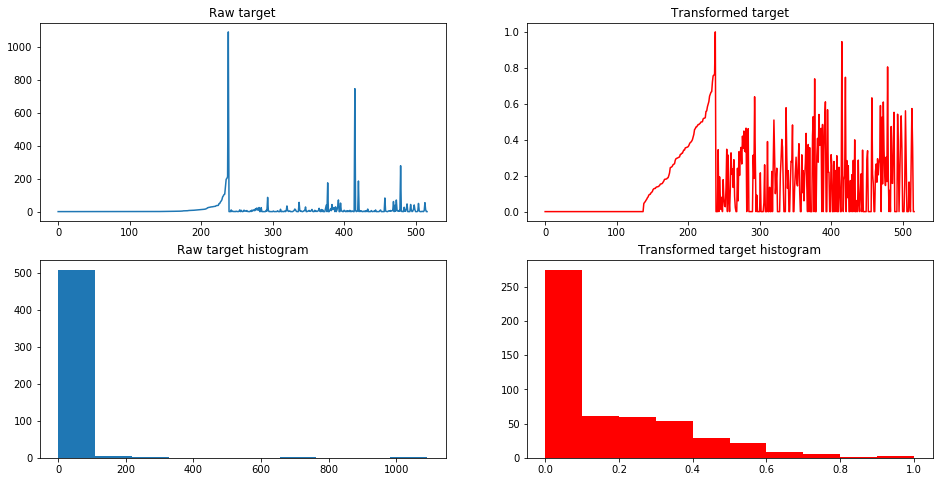
\includegraphics[width=\textwidth]{figures/target_transformation.png}
        \caption{Transformación del \emph{target}.}
        \label{fig:target_transform}
      \end{figure}
            
    \section{Desarrollo}
    
      Como se mencionó anteriormente, el enfoque de este proyecto será probar distintos modelos para 
      intentar obtener resultados mejores o comparables al trabajo realizado por la publicación guía. 
      Para apoyar el trabajo experimental se entrega un breve marco teórico sobre los modelos y métricas 
      utilizadas, para posteriormente detallar el proceso experimental y resultados del proyecto.
      
      \subsection{Modelos}
      
        A continuación se presenta una breve descripción de los modelos utilizados en el desarrollo 
        de este trabajo.
    
        \subsubsection{Regresión Lineal}
        
          La Regresión Lineal (\emph{Linear Regression} LR) es un modelo matemático que expresa el 
          valor predicho como la combinación lineal de los atributos de entrada \cite{seal1967studies}. 
          La notación matemática para un modelo de $I$ atributos es
      
          \begin{equation}
            \hat{y}(w, x) = \sum_{i=0}^{I} w_i x_i = Xw
          \end{equation}
          
          con $x_0=1$. La forma más común para resolver este problema es utilizando mínimos cuadrados 
          ordinarios
          
          \begin{equation}
            \underset{w}{\min\,} {|| X w - y||_2^2}
          \end{equation}
            
        \subsubsection{Arboles de Decisión}
        
          Los árboles de decisión (\emph{Decision Tree} DT) \cite{breimanolshen} son un tipo de modelos 
          construidos en base 
          a reglas lógicas que permiten representar y categorizar una serie de condiciones utilizadas 
          para resolver un problema. Se formalizan de la siguiente manera, dado un vector de entrenamiento 
          $x_i \in R^n, ~ i=1, ..., l$ y un vector de etiquetas $y \in \mathbb{R}^l$, un árbol de decisión
          particiona recursivamente el espacio de tal forma que las muestras con las mismas etiquetas 
          sean agrupadas conjuntamente. \medskip

          Sea $Q$ el dato contenido en el nodo $m$. Para cada candidato a división $\theta = (j, t_m)$ 
          consistente de una característica $j$ y un umbral $t_m$, particiona los datos en $Q_{\text{izq}}(\theta)$ 
          y $Q_{\text{der}}(\theta)$ subconjuntos
          
          \begin{equation}
            Q_{\text{izq}}(\theta) = (x, y) | x_j \leq t_m
          \end{equation}
          
          \begin{equation}
            Q_{\text{der}}(\theta) = Q \setminus Q_{left}(\theta)
          \end{equation}
          
          
          La impureza en $m$ es calculada utilizando una función de impureza $H()$, decisión que depende 
          del tipo de problema (clasificación o regresión)

          \begin{equation}
            G(Q, \theta) = \frac{n_{\text{izq}}}{N_m} H(Q_{\text{izq}}(\theta)) + \frac{n_{\text{der}}}{N_m} 
              H(Q_{\text{der}}(\theta)).
          \end{equation}            
          
          
          Los parámetros que minimizan la impureza se seleccionan de la siguiente forma
          
          \begin{equation}
            \theta^* = \operatorname{argmin}_\theta  G(Q, \theta).
          \end{equation}
         
          El procedimiento se repite recursivamente para los subconjuntos $Q_{\text{izq}}(\theta^*)$ y 
          $Q_{\text{der}}(\theta^*)$ hasta que la profundidad máxima definida haya sido alcanzada, 
          $N_m < \min_{\text{muestras}}$ o $N_m = 1$. \medskip
          
          Si el \emph{target} es un valor continuo (problemas de regresión), el nodo $m$ representa 
          una región $R_m$ con $N_m$ observaciones, los criterios utilizados puede ser el MSE, que minimiza 
          el error L2 utilizando la media de valores en los nodos terminales, o el MAE, que minimiza el 
          error L1 utilizando la mediana de los nodos terminales. De esta forma el MSE se define como
      
          \begin{equation}
            c_m = \frac{1}{N_m} \sum_{i \in N_m} y_i
          \end{equation}
          \begin{equation}
            H(X_m) = \frac{1}{N_m} \sum_{i \in N_m} (y_i - c_m)^2
          \end{equation}
          
          y el MAE como,
          
          \begin{equation}
            \bar{y_m} = \frac{1}{N_m} \sum_{i \in N_m} y_i
          \end{equation}
          \begin{equation}
            H(X_m) = \frac{1}{N_m} \sum_{i \in N_m} |y_i - \bar{y_m}|
          \end{equation}
          
          donde $X_m$ es el conjunto de entrenamiento en el nodo $m$.
                            
        \subsubsection{Máquinas de Soporte Vectorial}
        
          Las Máquinas de Soporte Vectorial (\emph{Support Vector Machines} SVM) \cite{Cortes1995} son una familia de modelos 
          que construyen uno o varios hiperplanos separadores en un espacio de alta dimensión para resolver 
          problemas de clasificación o regresión. \medskip
          
          Dado un conjunto de vectores de entrenamiento $x_i \in \mathbb{R}^p, i=1, ..., n$, y un vector 
          $y \in \mathbb{R}^n$, $\varepsilon$-SVR resuelve el siguiente problema primal:
          
          \begin{equation}
            \min_ {w, b, \zeta, \zeta^*} \frac{1}{2} w^T w + C \sum_{i=1}^{n} (\zeta_i + \zeta_i^*) 
            \nonumber
          \end{equation}
          \begin{equation}
            \begin{split}
              \textrm {sujeto a } & y_i - w^T \phi (x_i) - b \leq \varepsilon + \zeta_i,\\
                & w^T \phi (x_i) + b - y_i \leq \varepsilon + \zeta_i^*,\\
                & \zeta_i, \zeta_i^* \geq 0, i=1, ..., n
            \end{split}
          \end{equation}

          Su representación dual está dada por
          
          \begin{equation}
            \min_{\alpha, \alpha^*} \frac{1}{2} (\alpha - \alpha^*)^T Q (\alpha - \alpha^*) 
              + \varepsilon e^T (\alpha + \alpha^*) - y^T (\alpha - \alpha^*)
            \nonumber
          \end{equation}
          \begin{equation}
            \begin{split}
              \textrm {sujeto a } & e^T (\alpha - \alpha^*) = 0 \\
                & 0 \leq \alpha_i, \alpha_i^* \leq C, i=1, ..., n
            \end{split}
          \end{equation}

          donde $e$ es un vector de unos, $C > 0$ es la cota superior, $Q$ es una matriz semidefinida 
          positiva de dimensión $n \times n$, $Q_{ij} \equiv K(x_i, x_j) = \phi (x_i)^T \phi (x_j)$ es 
          el kernel. Implícitamente los vectores de entrenamiento son mapeados en un espacio de mayor 
          dimensionalidad (posiblemente infinita) por la función $\phi$. \\
          
          La función de decisión está definida por:
          
          \begin{equation}
            \sum_{i=1}^n (\alpha_i - \alpha_i^*) K(x_i, x) + \rho
          \end{equation}
          
          donde $\alpha_i - \alpha_i^*$ representa la diferencia de los vectores de soporte y $\rho$ 
          es el término independiente o intercepto. \\
          
          Las funciones de kernel utilizados en este tipo de problemas pueden ser los siguientes:
          \begin{itemize}
            \item Lineal: $\langle x, x'\rangle$.
            \item Polinomial: $(\gamma \langle x, x'\rangle + r)^d$. $d$ corresponde al grado del 
              polinomio, $\gamma$ y $r$ son parámetros.
            \item RBF: $\exp(-\gamma \|x-x'\|^2)$. $\gamma\geq 0$ es un parámetros.
            \item Sigmoide: $\tanh(\gamma \langle x,x'\rangle + r)$, con $\gamma$ y $r$ parámetros.
          \end{itemize}
                
            
        \subsubsection{Perceptrón Multicapa}
            
          El Perceptrón Multicapa (\emph{Multi-layer Perceptron} MLP) \cite{rumelhart1986learning}
           es un algoritmo de aprendizaje 
          supervisado que intenta aprender una función $f(\cdot): R^m \rightarrow R^o$ mediante el 
          entrenamiento sobre un \emph{dataset}, donde $m$ es la dimensión de la entrada y $o$
          es la dimensión de la salida. Dado un conjunto de características $X = {x_1, x_2, ..., x_m}$ 
          y su respectivo \emph{target} $y$, este algoritmo puede aprender una aproximador no lineal 
          ya sea para problemas de clasificación o regresión. \medskip
          
          Dado un conjunto de entrenamiento $\{(x_1, y_1), (x_2, y_2), \ldots, (x_n, y_n)\}$ donde 
          $x_i \in \mathbb{R}^n$ e $y_i \in \mathbb{R}$, una MLP de una capa oculta y una neurona 
          aprende la función $f(x) = W_2 ~ g(W_1^T x + b_1) + b_2$ donde $W_1 \in \mathbb{R}^m$ y 
          $W_2, b_1, b_2 \in \mathbb{R}$ son parámetros del modelo. $W_1, W_2$ representan los 
          pesos de la capa de entrada y oculta respectivamente; y $b_1, b_2$ representan los sesgos 
          añadidos a las capas ocultas y de salida respectivamente. $g(\cdot): \mathbb{R} \rightarrow \mathbb{R}$ 
          es la función de activación de la capa oculta. Generalmente en problemas de regresión, 
          la función de activación utilizada en la capa de salida es la función identidad. \medskip
            
          Siguiendo en problemas de regresión, el MLP utiliza como función de costo el Error Cuadrático 
          definido como,
          
          \begin{equation}
            Loss(\hat{y},y,W) = \frac{1}{2}||\hat{y} - y ||_2^2 + \frac{\alpha}{2} ||W||_2^2.
          \end{equation}

          Iniciando de un conjunto de pesos aleatorios el MLP minimiza la función de pérdida mediante 
          la actualización repetida de estos pesos. Luego de calcular la pérdida, se realiza un paso de 
          retropropagación desde la capa de salida hacia las capas anteriores, entregando a cada peso un 
          valor que corresponda a disminuir el valor de la función de pérdida en el proceso de actualización. \medskip

          En el gradiente descendente, el algoritmo de optimización generalmente utilizado, el gradiente 
          $\nabla Loss_{W}$  de la pérdida con respecto a los pesos, es calculada y derivada desde $W$. 
          Formalmente esto se expresa como,

          \begin{equation}
            W^{i+1} = W^i - \epsilon \nabla {Loss}_{W}^{i}
          \end{equation}
              
          donde $i$ es el paso de la iteración, y $\epsilon > 0$ es la tasa de aprendizaje. El algoritmo 
          se detiene una vez que alcanza el número máximo de iteraciones establecido o cuando se alcanza 
          una cierta tolerancia del error. \medskip
          
          Algunas funciones de activación típicas son:
          \begin{itemize}
            \item Identidad: $f(x)=x$
            \item Logística: $f(x)=\frac{1}{1+e^{-x}}$
            \item Tangente hiperbólica: $f(x)=\tanh(x)=\frac{e^x - e^{-x}}{e^x + e^{-x}}$
            \item Rectificador: (\emph{Rectified linear unit} ReLU): 
              $f(x)=\begin{cases} 0 & \text{para } x < 0 \\ x & \text{para } x \geq 0 \end{cases}$ 
          \end{itemize}
              
            
        % BAGGING
        \subsubsection{Bagging}
        
          El Bootstrap Aggregating (\emph{Bagging}) \cite{breiman1996bagging} es un algoritmo que busca mejorar los resultados 
          de predicción mediante la combinación de estimadores sobre datos de entrenamiento obtenidos 
          de forma aleatoria utilizando \emph{Bootstrap}. Formalmente podemos definir el método de la 
          siguiente forma, sea un conjunto de entrenamiento $S=\{(x_1, y_1), ...,  (x_m, y_m)\}$, para 
          $n=\{1, ..., N\}$ se genera una muestra \emph{Bootstrap} $S^n$ del conjunto $S$ y se entrena 
          un estimador $f_n$ utilizando esta muestra. Finalmente la función hipótesis del ensamblado 
          queda definida como:
          \begin{equation}
              F(\textbf{x}) = \frac1N \sum_{i=1}^N f_n(\textbf{x}).
          \end{equation}
                
                
        \subsubsection{Random Forest}
        
          \emph{Random Forest} (RF) \cite{breiman2001random} es una adaptación del algoritmo \emph{Bagging} en el cual se promedia 
          una gran cantidad de árboles de-correlacionados. Dado un conjunto de entrenamiento 
          $S=\{(x_1, y_1), ..., (x_m, y_m)\}$, para cada $n=\{1, ..., N\}$ se entrena un árbol $T_n$ 
          utilizando una muestra \emph{Bootstrap} $S^n$, repitiendo los siguientes pasos:
          \begin{enumerate}
            \item Seleccionar $j$ variables aleatoriamente desde los atributos $I$.
            \item Entrenar un árbol de clasificación o regresión (según corresponda) utilizando las 
              $j$ variables seleccionadas en (1).
          \end{enumerate}
          
          Esto se realiza para cada nodo terminal del árbol hasta alcanzar el número mínimo de nodos 
          $n_{min}$. Finalmente la hipótesis del ensamblado queda definida como:          
          \begin{equation}
            F(\textbf{x}) = \frac1N \sum_{n=1}^N T_n(\textbf{x}).
          \end{equation}
          
          Además del RF, también se probará una variante de este método denominada 
          \emph{Extremely Randomized Tree} (ET) \cite{geurts2006extremely}, en donde la regla de división de los árboles se 
          construye de forma aleatoria.%que incluye aleatoriedad al momento de definir los umbrales de 
          %división para los atributos candidatos. 

                        
        % BOOSTING    
        \subsubsection{Boosting}
            
          Los algoritmos de tipo \emph{Boosting} \cite{freund1997decision} intentan mejorar la predicción de un modelo mediante 
          la iteración sobre \emph{weak learners} para luego, mediante la agregación de estos, construir 
          un modelo más robusto. La implementación utilizada en este trabajo es el algoritmo \emph{AdaBoost}, 
          específicamente \emph{AdaBoost.R2} \cite{drucker1997improving} el cual funciona de la siguiente 
          forma, inicializar los pesos $w_i=1, ~ i=1,...,N_1$, para cada muestra de entrenamiento. 
          Repetir los siguientes pasos hasta que el promedio de la función de pérdida sea menor a $0.5$:
          \begin{enumerate}
            \item Obtener una muestra de $N_1$ ejemplos (con reemplazo) para generar el conjunto de 
              entrenamiento. La probabilidad de que un ejemplo $i$ esté dentro del conjunto de entrenamiento 
              es $p_i=\frac{w_i}{\sum w_i}$
            \item Construir un estimador para generar la hipótesis $h_t: x \rightarrow y$.
            \item Entrenar el estimador para obtener la predicción $y_i^{(p)}(\textbf{x}_i), ~ i=1, ..., N$.
            \item Calcular el error $L_i$ para cada ejemplo de entrenamiento.
            \item Calcular el error promedio $\bar{L}=\sum_{i=1}^{N_1}L_ip_i$.
            \item Definir $\beta=\frac{\bar{L}}{1-\bar{L}}$, donde $\beta$ es una medida de confianza del 
              predictor. Un bajo $\beta$ indica alta confianza.
            \item Actualizar los pesos $w_i\rightarrow w_i\beta^{1-L_i}$
          \end{enumerate}
            
          Para una entrada $\textbf{x}_i$ cada una de los $T$ estimadores generan una predicción 
          $h_t, ~ t=1, ..., T$. La predicción acumulada $h_f$ utilizando $T$ estimadores se define como
          \begin{equation}
            h_f = \inf \left\{y\in Y: ~ \sum_{t:h_t\leq y} \log(1/\beta_t) \geq \frac12 \sum_{t} \log(1/\beta_t) \right\}.
          \end{equation}
          
          Las funciones de pérdida $L_i$ a utilizar pueden ser:
          \begin{itemize}
            \item Lineal: $L_i=\frac{|y_i^{(p)}(\textbf{x}_i)-y_i|}{D}$
            \item Cuadrática: $L_i=\frac{|y_i^{(p)}(\textbf{x}_i)-y_i|^2}{D^2}$
            \item Exponencial: $L_i=1- \exp\left(\frac{-|y_i^{(p)}(\textbf{x}_i)-y_i|}{D}\right)$
          \end{itemize}
          
          donde $D=\sup|y_i^{(p)}(\textbf{x}_i)-y_i|, ~ i=1, ..., N_1$
                
            
        \subsubsection{Gradient Tree Boosting}
        
          \emph{Gradient Tree Boosting} (GTB) \cite{friedman2001greedy} es una generalización de la técnica \emph{Boosting} pero que 
          puede utilizar una función de costo diferenciable arbitraria. GTB es un método considerablemente 
          más preciso y efectivo que puede ser utilizado para problemas de regresión
          y clasificación. \medskip
          
          La formulación matemática de este modelo es la siguiente, GTB considera la suma de modelos de 
          la siguiente forma:
          \begin{equation}
            F(x) = \sum_{m=1}^{M} \gamma_m h_m(x)
          \end{equation}
          
          donde $h_m(x)$ son funciones base denominadas generalmente como \emph{weak learners} en el 
          contexto de \emph{Boosting}. GTB utiliza árboles de decisión de tamaño fijo como \emph{weak learners}. 
          Los árboles de decisión tienen un número de habilidades que permiten que sean útiles para 
          el \emph{boosting}, por ejemplo la capacidad de manipular datos de distinto tipo además de 
          modelar funciones de alta complejidad. \medskip

          Al igual que otros algoritmos de \emph{Boosting}, GTB construye modelos aditivos de forma secuencial:
          
          \begin{equation}
            F_m(x) = F_{m-1}(x) + \gamma_m h_m(x).
          \end{equation}
           
          En cada etapa, el árbol de decisión $h_m(x)$ es escogido de forma que minimice la función de pérdida 
          $L$ dado el modelo actual $F_{m-1}$ y su ajuste $F_{m-1}(x_i)$
          \begin{equation}
            F_m(x) = F_{m-1}(x) + \arg\min_{h} \sum_{i=1}^{n} L(y_i, F_{m-1}(x_i) + h(x))
          \end{equation}
           
          El modelo inicial $F_{0}$ es específico del problema, por ejemplo para una regresión por mínimos 
          cuadrados, por lo general, se escoge la media de los valores de \emph{target}. \medskip
          
          GTB intenta resolver el problema de minimización numéricamente por medio de gradiente descendente: 
          La dirección corresponde al gradiente  negativo del la función de costo evaluada en el modelo actual 
          $F_{m-1}$ el cual puede ser calculado para cualquier función de costo diferenciable de la siguiente forma:

          \begin{equation}
            F_m(x) = F_{m-1}(x) - \gamma_m \sum_{i=1}^{n} \nabla_F L(y_i, F_{m-1}(x_i)),
          \end{equation}
          
          donde el tamaño del paso $\gamma_m$ se escoge utilizando una búsqueda lineal:
          
          \begin{equation}
            \gamma_m = \arg\min_{\gamma} \sum_{i=1}^{n} L\left(y_i, F_{m-1}(x_i) - 
              \gamma \frac{\partial L(y_i, F_{m-1}(x_i))}{\partial F_{m-1}(x_i)}\right)
          \end{equation}
           
          El algoritmo para regresión o clasificación solo se diferencian en la función de pérdida utilizada. 
          Para el caso de regresión, algunas de las funciones de pérdida utilizadas son:
          \begin{itemize}
            \item Mínimos cuadrados $L = \sum_{i=1}^n (y_i - f(x_i))^2$.
            \item Mínimas desviaciones absolutas $L = \sum_{i=1}^n |y_i - f(x_i)|$.
            \item La función de Huber $L = \sum_{i=1}^n L_{\delta}(y_i, f(x_i)), ~ 
              L_{\delta }(y,f(x))=\begin{cases}{\frac  {1}{2}}(y-f(x))^{2} & {\textrm{para }}|y-f(x)|\leq 
              \delta ,\\ \delta \,|y-f(x)|-{\frac  {1}{2}}\delta ^{2} & {\textrm{en otro caso.}}\end{cases}$
          \end{itemize}
            
        
      % METRICS
      \subsection{Métricas}
      
        Las métricas utilizadas para el análisis de los modelos fueron los siguientes:
        
        \iffalse
        % R2
        \subsubsection{Coeficiente de Determinación}
        
          El Coeficiente de Determinación ($R^2$), proporciona una medida de que tan bien es probable 
          que las futuras muestras sean predichas por el modelo. El mejor puntaje es $1.0$ y puede ser 
          negativo en el caso que el modelo sea malo. Un modelo que siempre prediga el valor esperado 
          de $y$, sin tomar en cuenta las características de entrada, otendrá un $R^2=0$. Se define de 
          la siguiente forma, si $\hat{y}_i$ es el valor predicho de la $i$-ésima muestra e $y_i$ es el 
          valor real correspondiente, entonces el $R^2$ estimado sobre $N$ muestras se define como
          
          \begin{equation}
            R^2(y, \hat{y}) = 1 - \frac{\sum_{i=1}^{N} (y_i - \hat{y}_i)^2}{\sum_{i=1}^{N} (y_i - \bar{y})^2}
          \end{equation}

          donde $\bar{y} =  \frac{1}{N} \sum_{i=1}^{N} y_i$.
          \fi
          
        % MSE
        \subsubsection{Error Cuadrático Medio}
        
          El Error Cuadrático Medio (\emph{Mean Squared Error} MSE) es una métrica que corresponde al 
          valor esperado del error o pérdida al cuadrado. Se define de la siguiente forma, si $\hat{y}_i$ 
          es el valor predicho de $i$-ésimo ejemplo, e $y_i$ corresponde al valor verdadero, entonces
          el MSE estimado sobre $N$ muestras está definido por
          
          \begin{equation}
            \text{MSE}(y, \hat{y}) = \frac{1}{N} \sum_{i=1}^{N} (y_i - \hat{y}_i)^2.
          \end{equation}

          Para comparar con los resultados expuestos en el artículo guía, se incluye también el
          $RMSE$ que es la raíz cuadrada del $MSE$.
          
        % MAE
        \subsubsection{Error Medio Absoluto}
        
          El Error Medio Absoluto (\emph{Mean Absolute Error} MAE) es una métrica que corresponde al valor 
          esperado de la pérdida de valor absoluto o norma $L1$. Se define de la siguiente manera, si 
          $\hat{y}_i$ es el valor predicho del $i$-ésimo ejemplo, y $y_i$ es el valor real correspondiente, 
          entonces el MAE estimado sobre $N$ muestras está definido por
          
          \begin{equation}
            \text{MAE}(y, \hat{y}) = \frac{1}{N} \sum_{i=1}^{N} \left| y_i - \hat{y}_i \right|.
          \end{equation}

  
      % EXPERIMENTS    
      \subsection{Experimentos}
      
        \iffalse
        Dada la variedad de modelos que se desean probar es que se proponen distintas combinaciones de 
        características y transformaciones de la variable dependiente. La principal justificación de este 
        pre-procesamiento tiene relación a la baja cantidad de datos que existen en el \emph{dataset} de 
        estudio. Por esto último es que también el análisis de todo este trabajo se realiza sobre un 
        análisis de \emph{K-Fold cross validation} con un valor de $K=5$. \medskip
        
        Los características del \emph{dataset} se combinaron de la siguiente forma:
        \begin{enumerate}
          \item $X$ corresponde a todos los atributos del \emph{dataset}.
          \item $X1C$ corresponde a todos los atributos del \emph{dataset}, codificando las variables 
            categóricas.
          \item $STFWI$ corresponde a utilizar los datos espaciales, temporales y FWI del \emph{dataset}.
          \item $STFWI1C$ corresponde a los datos espaciales, temporales y FWI del \emph{dataset}, 
            codificando las variables categóricas.
          \item $STM$ corresponde a los datos espaciales, temporales y meteorológicos.
          \item $STM1C$ corresponde a los datos espaciales, temporales y meteorológicos, codificando las 
            variables categóricas.
          \item $FWI$ corresponde a los datos de este sistema Canadiense.
          \item $M$ corresponde solo a utilizar los datos meteorológicos.
        \end{enumerate}
        
        Cada uno de estos conjuntos fueron estandarizados, es decir, se restó la media y dividió por la varianza 
        de cada atributo.
        
        Los datos de \emph{target} fueron probados de tres formas distintas:
        \begin{enumerate}
          \item Utilizando normalización entre $[0, 1]$.
          \item Aplicando la transformación logarítmica $y=\ln(x+1)$.
          \item Aplicando la transformación logarítmica y además normalizar el resultado al rango $[0, 1]$.
        \end{enumerate}
        
        Para ajustar los hiper-parámetros de cada modelo se utilizó una búsqueda exhaustiva implementada como 
        \emph{Grid Search} con \emph{Cross-Validation}. Además, se incluyen las combinaciones de características 
        y \emph{targets}. Entre cada familia de modelos se escogió el de mejor valor de $R^2$.
        \fi

        Para el desarrollo de este trabajo se dividió el \emph{dataset} en un conjunto de entrenamiento y prueba, en 
        la proporción $80\%$ y $20\%$ respectivamente. En el ajuste de los hiper-parámetros de cada modelo se utilizó 
        una búsqueda exhaustiva implementada como \emph{Grid Search} con \emph{Cross-Validation} con $K=5$. Entre cada familia 
        de modelos se escogió el de menor valor de $MSE$ resultante del \emph{Cross-Validation} sobre el conjunto de
        entrenamiento. Una vez seleccionado el modelo, se aplicaron las métricas sobre el conjunto de prueba.
          
        
      % RESULTS
      \subsection{Resultados}
      
        %TODO
        % \begin{table}[!ht]
        %     \centering
        %     \caption{Mejores resultados para cada modelo}
        %     \label{tab:results}
        %     \begin{tabular}{l|rr}
        %         \hline
        %         Model    & MSE    & MAE    \\ \hline \hline
        %         LR       & 0.041  & 0.167  \\
        %         DT       & 0.002  & 0.013  \\
        %         SVM      & 0.003  & 0.015  \\
        %         MLP      & 0.042  & 0.172  \\
        %         Bagging  & 0.043  & 0.172  \\
        %         RF       & 0.002  & 0.016  \\ 
        %         ET       & 0.003  & 0.013  \\
        %         Adaboost & 0.041  & 0.171  \\
        %         GBT      &        &        \\ \hline
        %     \end{tabular}
        % \end{table}

        A continuación se presentan los resultados obtenidos luego de los experimentos.

        \clearpage

        \begin{table}[!ht]
          \centering
          \caption{Resultado de las méticas para cada modelo}
          \label{tab:results}
          \begin{tabular}{l|rrr}
            \hline
            Model    & MSE   & RMSE & MAE \\ \hline \hline
            LR       & 12069.92 & 109.86 & 19.58 \\
            DT       & 11575.84 & 107.59 & 15.02 \\
            SVM      & 12135.25 & 110.16 & 19.67 \\
            MLP      & 12079.37 & 109.91 & 19.66 \\
            Bagging  & 8978.24  & 94.75  & 14.38 \\
            RF       & 10293.97 & 101.46 & 15.25 \\ 
            ET       & 11764.26 & 108.46 & 18.04 \\
            Adaboost & 11957.46 & 109.35 & 19.65 \\
            GTB      & 4255.87  & 65.24  & 8.13  \\ \hline
          \end{tabular}
        \end{table}        

        De los resultados obtenidos podemos corroborar que son comparables a los expuestos en el 
        artículo que se utilizó como base. Es importante mencionar que el resultado del
        \emph{GTB} fue mejor que los resultados del artículos en términos del $MAE$.
  
    
    % CONCLUSIONS
    \section{Conclusiones}
        
      Del desarrollo de este proyecto notamos la potencia de los modelos ensamblados, los cuales
      mejoran los resultados considerablemente en comparación a los modelos no ensamblados. El principal
      problema de estos modelos es que tienden a sobreajustar, pero gracias al uso de algunas herramientas
      (según el modelo) se puede mitigar este problema. Si bien, la publicación guía sugiere el uso de 
      ciertas configuraciones de $X$, que podría ser vistos como una selección de características, el 
      modelo \emph{GTB} demostró mejorar los resultados utilizando toda la información. \medskip

      Por limitaciones computacionales no se realizaron más pruebas, pero como trabajo futuro
      se espera incluir técnicas de selección de características para así poder comparar resultados
      en iguales condiciones al artículo guía. \medskip

      El modelo \emph{GTB} nos entregó resultados bastante interesantes sobre los modelos que se utilizan 
      el artículo. Según la literatura es uno de los modelos más potentes pero que lamentablemente tiene 
      asociada una alta exigencia computacional dada la estructura iterativa del algoritmo. De todas 
      formas gracias a las capacidades computacionales actuales este podría no ser un inconveniente, 
      siempre que el problema no implique re-entrenar el modelo muchas veces o quizás el uso de 
      entrenamiento en tiempo real.

	% REFERENCES
  \bibliographystyle{apacite}
  \bibliography{references}

\end{document}
